\documentclass{assignment}
\ProjectInfos{高等量子力学}{PHYS5001P}{2022-2023 学年第一学期}{第四次作业}{截止时间: 2022 年 10 月 17 日 (周一)}{陈稼霖}[https://github.com/Chen-Jialin]{SA21038052}

\begin{document}
\begin{prob}[课本习题 2.24]
    考虑一维粒子被一个 $\delta$ 函数势
    \[
        V(x)=-\nu_0\delta(x),\quad(\nu_0\text{ 为正实数})
    \]
    束缚于一个固定的中心位置处, 求波函数和基态束缚能. 有激发的束缚态吗?
\end{prob}
\begin{prob}
    该粒子的哈密顿量为
    \begin{align}
        H=\frac{p^2}{2m}+V(x)=\left\{\begin{array}{ll}
            \frac{p^2}{2m},&x\neq 0,\\
            \frac{p^2}{2m}-\nu_0\delta(x),&x=0.
        \end{array}\right.
    \end{align}
    在 $x\neq 0$ 处的薛定谔方程为
    \begin{align}
        -\frac{\hbar^2}{2m}\frac{\partial^2\psi}{\partial x^2}=E\psi.
    \end{align}
    考虑到束缚态波函数在无穷远处的函数值为 $0$, $x<0$ 处和 $x>0$ 处波函数的通解分别为
    \begin{align}
        \psi(x<0)=Ae^{kx},\\
        \psi(x>0)=Be^{-kx},
    \end{align}
    其中 $k=\frac{\sqrt{2mE}}{\hbar}$.
    利用连续性条件
    \begin{gather}
        \psi(x=0^-)=A=\psi(x=0^+)=B,\\
        \psi'(x=0^+)-\psi'(x=0^-)=-Ak-Bk=\int_{0^-}^{0^+}\frac{\partial^2\psi}{\partial x'^2}\,\mathrm{d}x'=\frac{2m}{\hbar^2}\int_{0^-}^{0^+}[-\nu_0\delta(x)-E]\psi(0)\,\mathrm{d}x'=-\frac{2m\nu_0}{\hbar^2}A,
    \end{gather}
    解得
    \begin{align}
        A=B,\quad k=\frac{m\nu_0}{\hbar^2}.
    \end{align}
    考虑到波函数满足归一化条件, 得波函数
    \begin{align}
        \psi(x)=\frac{\sqrt{m\nu_0}}{\hbar}e^{-m\nu_0\abs{x}/\hbar^2},
    \end{align}
    基态束缚能为
    \begin{align}
        E=\frac{\hbar^2\Omega^2}{2m}.
    \end{align}

    该系统仅有一个束缚基态, 没有激发的束缚态
\end{prob}

\begin{prob}[课本习题 2.26]
    一个一维粒子 ($-\infty<x<\infty$) 受到一个可从
    \[
        V=\lambda x,\quad(\lambda>0)
    \]
    导出的恒力的作用.
    \begin{itemize}
        \item[(a)] 其能谱是连续的还是分立的? 写出由 $E$ 所确定的能量本征函数的近似表达式. 然后粗略地画出其示意图.
        \item[(b)] 简略地讨论, 如果用
        \[
            V=\lambda\abs{x}.
        \]
        代替 $V$, 什么地方需要改动?
    \end{itemize}
\end{prob}
\begin{sol}
    \begin{itemize}
        \item[(a)] 在 $x\rightarrow-\infty$ 处必有 $E>V$, 粒子非束缚, 故其能谱必为连续的.

        能量本征函数的近似表达式为
        \begin{align}
            \psi(x)\sim\left\{\begin{array}{ll}
                \frac{1}{[E-\lambda x]^{1/4}}e^{\pm\frac{i}{\hbar}\int_{-\infty}^x\sqrt{2m(E-\lambda x')}\,\mathrm{d}x'},&\text{for }x<\frac{E}{\lambda},\\
                \frac{1}{[\lambda x-E]^{1/4}}e^{-\frac{1}{\hbar}\int_{E/\lambda}^x\sqrt{2m(\lambda x'-E)}\,\mathrm{d}x'},&\text{for }x>\frac{E}{\lambda}.
            \end{array}\right.
        \end{align}
        如图 \ref{4-1} 所示.
        \begin{figure}[H]
            \centering
            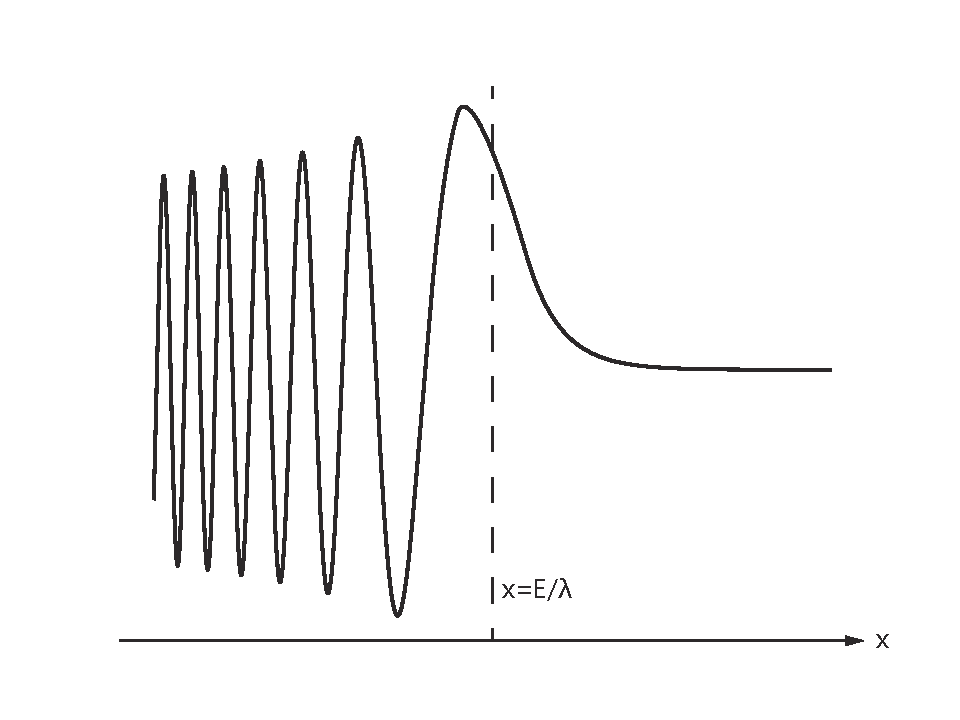
\includegraphics[width=.5\columnwidth]{4-1.pdf}
            \caption{能量本征函数的近似图像. 注意在 $x<E/\lambda$ 处波函数为波动形式, 且随着 $x\rightarrow-\infty$, 波动频率加快, 波动幅度变小; 在 $x>E/\lambda$ 处波函数为衰减形式.}
            \label{4-1}
        \end{figure}
        \item[(2)] 若 $V=\lambda\abs{x}$, 则粒子处于束缚态, 能谱为一系列分离的本征能量构成. 能量本征函数的近似表达式为
        \begin{align}
            \psi(x)\sim\left\{\begin{array}{ll}
                \frac{1}{[-\lambda x-E]^{1/4}}e^{\frac{1}{\hbar}\int_{-\infty}^x\sqrt{2m(-\lambda x'-E)}\,\mathrm{d}x'},&\text{for }x<-\frac{E}{\lambda},\\
                \frac{1}{[E-\lambda\abs{x}]^{1/4}}\cos\left[\frac{1}{\hbar}\int_{-E/\lambda}^x\sqrt{2m(E-\lambda\abs{x'})}\,\mathrm{d}x'\right],&\text{for }-\frac{E}{\lambda}<x<\frac{E}{\lambda},\\
                \frac{1}{[\lambda x-E]^{1/4}}e^{-\frac{1}{\hbar}\int_{E/\lambda}^x\sqrt{2m(\lambda x'-E)}\,\mathrm{d}x'},&\text{for }x>\frac{E}{\lambda},
            \end{array}\right.
        \end{align}
        或
        \begin{align}
            \psi(x)\sim\left\{\begin{array}{ll}
                \frac{1}{[-\lambda x-E]^{1/4}}e^{\frac{1}{\hbar}\int_{-\infty}^x\sqrt{2m(-\lambda x'-E)}\,\mathrm{d}x'},&\text{for }x<-\frac{E}{\lambda},\\
                \frac{1}{[E-\lambda\abs{x}]^{1/4}}\sin\left[\frac{1}{\hbar}\int_{-E/\lambda}^x\sqrt{2m(E-\lambda\abs{x'})}\,\mathrm{d}x'\right],&\text{for }-\frac{E}{\lambda}<x<\frac{E}{\lambda},\\
                \frac{1}{[\lambda x-E]^{1/4}}e^{-\frac{1}{\hbar}\int_{E/\lambda}^x\sqrt{2m(\lambda x'-E)}\,\mathrm{d}x'},&\text{for }x>\frac{E}{\lambda},
            \end{array}\right.
        \end{align}
        这些本征函数均为偶函数或奇函数.
        能量本征值满足
        \begin{align}
            \int_{-E/\lambda}^{E/\lambda}\sqrt{2m(E-\lambda\abs{x'})}\,\mathrm{d}x'=(n+\frac{1}{2})\pi\hbar,\quad n=0,1,2,3,\cdots
        \end{align}
        解得能量本征值为
        \begin{align}
            E_n=\frac{\left[3\left(n+\frac{1}{4}\right)\pi\hbar\lambda\right]^{2/3}}{2m^{1/3}},\quad n=0,1,2,3,\cdots
        \end{align}
    \end{itemize}
\end{sol}

\begin{prob}[课本习题 2.31]
    导出 (2.6.16) 式, 并求得 (2.6.16) 式的三维推广.
\end{prob}
\begin{pf}
    一维自由粒子的哈密顿量为
    \begin{align}
        H=\frac{p^2}{2m},
    \end{align}
    显然其与动量算符 $p$ 对易; $\{\lvert p'\rangle\}$ 为哈密顿量 $H$ 和动量算符 $p$ 的共同本征态:
    \begin{align}
        p\lvert p'\rangle=p'\lvert p'\rangle,\quad H\lvert p'\rangle=\left(\frac{p'^2}{2m}\right)\lvert p'\rangle.
    \end{align}
    由传播子的定义, 一维自由粒子的传播子为
    \begin{align}
        \notag K(x'',t;x',t_0)=&\int_{-\infty}^{\infty}\mathrm{d}p'\,\langle x''\vert p'\rangle\langle p'\vert x'\rangle\exp\left[\frac{-iE_{p'}(t-t_0)}{\hbar}\right]\\
        \notag&(\text{利用 }\langle x'\vert p'\rangle=\frac{1}{\sqrt{2\pi\hbar}}\exp\left(\frac{ip'x'}{\hbar}\right))\\
        \notag=&\frac{1}{2\pi\hbar}\int_{-\infty}^{\infty}\mathrm{d}p'\,\exp\left[\frac{ip'(x''-x')}{\hbar}-\frac{ip'^2(t-t_0)}{2m\hbar}\right]\\
        \notag=&\frac{1}{2\pi\hbar}\int_{-\infty}^{\infty}\mathrm{d}p'\,\exp\left\{-\frac{i(t-t_0)}{2m\hbar}\left[p'-\frac{m(x''-x')}{t-t_0}\right]^2+\frac{im(x''-x')^2}{2\hbar(t-t_0)}\right\},\\
        \notag&(\text{令 }\xi'=\sqrt{\frac{i(t-t_0)}{2m\hbar}}\left[p'-\frac{m(x''-x')}{t-t_0}\right])\\
        \notag=&\frac{1}{2\pi\hbar}\sqrt{\frac{2m\hbar}{i(t-t_0)}}\int_{-\infty}^{\infty}\mathrm{d}\xi\,\exp(-\xi^2)\exp\left[\frac{im(x''-x')^2}{2\hbar(t-t_0)}\right],\\
        \notag&(\text{利用高斯积分 }\int_{-\infty}^{\infty}e^{-\xi^2}\,\mathrm{d}\xi=\sqrt{\pi})\\
        =&\sqrt{\frac{m}{2\pi i\hbar(t-t_0)}}\exp\left[\frac{im(x''-x')^2}{2\hbar(t-t_0)}\right],
    \end{align}
    此即 (2.6.16) 式.

    下面将上式推广至三维情况. 三维自由粒子的哈密顿量为
    \begin{align}
        H=\frac{p_x^2+p_y^2+p_z^2}{2m},
    \end{align}
    显然与动量算符 $p_x$, $p_y$, $p_z$ 对易; $\{\lvert p_x',p_y',p_z'\rangle\}$ 为哈密顿量 $H$ 和动量算符 $p_x$, $p_y$, $p_z$ 的共同本征态:
    \begin{gather}
        p_x\lvert p_x',p_y',p_z'\rangle=p_x'\lvert p_x',p_y',p_z'\rangle,\quad p_y\lvert p_x',p_y',p_z'\rangle=p_y'\lvert p_x',p_y',p_z'\rangle,\quad p_z\lvert p_x',p_y',p_z'\rangle=p_z'\lvert p_x',p_y',p_z'\rangle,\\
        H\lvert p_x',p_y',p_z'\rangle=\frac{p_x'^2+p_y'^2+p_z'^2}{2m}\lvert p_x',p_y',p_z'\rangle.
    \end{gather}
    由传播子的定义, 三维自由粒子的传播子为
    \begin{align}
        \notag K(\bm{x}'',t;\bm{x},t_0)=&\int_{-\infty}^{\infty}\mathrm{d}p_x'\int_{-\infty}^{\infty}\mathrm{d}p_y'\int_{-\infty}^{\infty}\mathrm{d}p_z'\,\langle\bm{x}''\vert p_x',p_y',p_z'\rangle\langle p_x',p_y',p_z'\vert\bm{x}'\rangle\exp\left[-\frac{iE_{p_x',p_y',p_z'}(t-t_0)}{\hbar}\right]\\
        \notag&(\text{利用 }\langle\bm{x}'\vert\bm{p}'\rangle=\frac{1}{(2\pi\hbar)^{3/2}}\exp\left(\frac{i\bm{p}'\cdot\bm{x}'}{\hbar}\right))\\
        \notag=&\frac{1}{(2\pi\hbar)^3}\int_{-\infty}^{\infty}\mathrm{d}p_x'\int_{-\infty}^{\infty}\mathrm{d}p_y'\int_{-\infty}^{\infty}\mathrm{d}p_z'\times\\
        \notag&\exp\left\{\frac{i[p_x'(x''-x')+p_y'(y''-y')+p_z'(z''-z')]}{\hbar}-\frac{i(p_x'^2+p_y'^2+p_z'^2)(t-t_0)}{2m\hbar}\right\}\\
        \notag=&\frac{1}{(2\pi\hbar)^3}\int_{-\infty}^{\infty}\mathrm{d}p_x'\,\exp\left\{-\frac{i(t-t_0)}{2m\hbar}[p_x'-\frac{m(x''-x')}{t-t_0}]^2+\frac{im(x''-x')}{2\hbar(t-t_0)}\right\}\times\\
        \notag&\int_{-\infty}^{\infty}\mathrm{d}p_y'\,\exp\left\{-\frac{i(t-t_0)}{2m\hbar}[p_y'-\frac{m(y''-y')}{t-t_0}]^2+\frac{im(y''-y')}{2\hbar(t-t_0)}\right\}\times\\
        \notag&\int_{-\infty}^{\infty}\mathrm{d}p_z'\,\exp\left\{-\frac{i(t-t_0)}{2m\hbar}[p_z'-\frac{m(z''-z')}{t-t_0}]^2+\frac{im(z''-z')}{2\hbar(t-t_0)}\right\}\\
        =&\left(\frac{m}{2\pi i\hbar(t-t_0)}\right)^{3/2}\exp\left\{\frac{im[(x''-x')^2+(y''-y')^2+(z''-z')^2]}{2\hbar(t-t_0)}\right\}.
    \end{align}
\end{pf}

\begin{prob}
    求一维自由粒子高斯波包坐标与动量测不准关系随时间的变化.
\end{prob}
\begin{sol}
    $t=0$ 时刻一维自由粒子高斯波包的波函数为
    \begin{align}
        \psi(x',0)=e^{ip_0x'/\hbar}\frac{\exp\left(-\frac{x'^2}{2d_0^2}\right)}{(\pi d_0^2)^{1/4}}.
    \end{align}
    一维自由粒子的传播子为
    \begin{align}
        K(x'',t;x',t_0)=\sqrt{\frac{m}{2\pi i\hbar(t-t_0)}}\exp\left[\frac{im(x''-x')^2}{2\hbar(t-t_0)}\right].
    \end{align}
    $t$ 时刻该波包的波函数演化为
    {\small
    \begin{align}
        \notag\psi(x,t)=&\int K(x,t;x',0)\psi(x',0)\,\mathrm{d}x'\\
        \notag=&\int_{-\infty}^{\infty}\sqrt{\frac{m}{2\pi i\hbar t}}\exp\left[\frac{im(x-x')^2}{2\hbar t}\right]e^{ip_0x'/\hbar}\frac{\exp\left(-\frac{x'^2}{2d_0^2}\right)}{(\pi d_0^2)^{1/4}}\,\mathrm{d}x'\\
        \notag=&\sqrt{\frac{m}{2\pi i\hbar t}}\frac{1}{(\pi d_0^2)^{1/4}}\int_{-\infty}^{\infty}\exp\left\{\left(\frac{im}{2\hbar t}-\frac{1}{2d_0^2}\right)x'^2-\left(\frac{imx}{\hbar t}-\frac{ip_0}{\hbar}\right)x'+\frac{imx^2}{2\hbar t}\right\}\,\mathrm{d}x'\\
        \notag=&\sqrt{\frac{m}{2\pi i\hbar t}}\frac{1}{(\pi d_0^2)^{1/4}}\int_{-\infty}^{\infty}\exp\left\{-\left(-\frac{im}{2\hbar t}+\frac{1}{2d_0^2}\right)\left[x'^2-2\frac{x-\frac{p_0t}{m}}{1+i\frac{\hbar t}{md_0^2}}+\frac{x^2}{1+i\frac{\hbar t}{md_0^2}}\right]\right\}\,\mathrm{d}x'\\
        \notag=&\sqrt{\frac{m}{2\pi i\hbar t}}\frac{1}{(\pi d_0^2)^{1/4}}\int_{-\infty}^{\infty}\exp\left\{-\left(-\frac{im}{2\hbar t}+\frac{1}{2d_0^2}\right)\left(x'-\frac{x-\frac{p_0t}{m}}{1+i\frac{\hbar t}{md_0^2}}\right)^2+\frac{-\frac{im}{2\hbar t}\left(x-\frac{p_0t}{m}\right)^2+\left(\frac{im}{2\hbar t}-\frac{1}{2d_0^2}\right)x^2}{1+\frac{i\hbar t}{md_0^2}}\right\}\,\mathrm{d}x'\\
        \notag&(\text{令 }\xi=\left(\frac{im}{2\hbar t}-\frac{1}{2d_0^2}\right)^{1/2}\left(x'-\frac{x-\frac{p_0t}{m}}{1+i\frac{\hbar t}{md_0^2}}\right))\\
        \notag=&\sqrt{\frac{m}{2\pi i\hbar t}}\frac{1}{(\pi d_0^2)^{1/4}}\left(-\frac{im}{2\hbar t}+\frac{1}{2d_0^2}\right)^{-1/2}\int_{-\infty}^{\infty}\exp\left\{-\xi^2+\frac{-\frac{im}{2\hbar t}\left(x-\frac{p_0t}{m}\right)^2+\left(\frac{im}{2\hbar t}-\frac{1}{2d_0^2}\right)x^2}{1+\frac{i\hbar t}{md_0^2}}\right\}\,\mathrm{d}\xi\\
        \notag&(\text{利用高斯积分 }\int_{-\infty}^{\infty}e^{-\xi^2}=\sqrt{\pi})\\
        \notag=&\left[\pi^{1/2}\left(d_0+\frac{i\hbar t}{md_0}\right)\right]^{-1/2}\exp\left[\frac{-\frac{im}{2\hbar t}\left(x-\frac{p_0t}{m}\right)^2+\left(\frac{im}{2\hbar t}-\frac{1}{2d_0^2}\right)x^2}{1+\frac{i\hbar t}{md_0^2}}\right]\\
        =&\left[\pi^{1/2}\left(d_0+\frac{i\hbar t}{md_0}\right)\right]^{-1/2}\exp\left[\frac{-\left(x-\frac{p_0t}{m}\right)^2\left(1-\frac{i\hbar t}{md_0^2}\right)}{2d_0^2\left(1+\frac{\hbar^2t^2}{m^2d_0^4}\right)}\right]\exp\left[\frac{ip_0}{\hbar}\left(x-\frac{p_0t}{2m}\right)\right].
    \end{align}
    }
    此时位置坐标的期望值为
    \begin{align}
        \langle x\rangle=\int_{-\infty}^{\infty}\psi^*(x',t)x\psi(x',t)\,\mathrm{d}x'=\frac{p_0t}{m}.
    \end{align}
    位置坐标的平方的期望值为
    \begin{align}
        \notag\langle x^2\rangle=&\int_{-\infty}^{\infty}\psi^*(x',t)x^2\psi(x',t)\,\mathrm{d}x'\\
        \notag=&\pi^{-1/2}\left(d_0^2+\frac{\hbar^2t^2}{m^2d_0^2}\right)^{-1/2}\int_{-\infty}^{\infty}\exp\left[\frac{-\left(x'-\frac{p_0t}{m}\right)^2}{d_0^2\left(1+\frac{\hbar^2t^2}{m^2d_0^4}\right)}\right]x'^2\,\mathrm{d}x'\\
        \notag=&\pi^{-1/2}\left(d_0^2+\frac{\hbar^2t^2}{m^2d_0^2}\right)^{-1/2}\int_{-\infty}^{\infty}\exp\left[\frac{-\left(x'-\frac{p_0t}{m}\right)^2}{d_0^2\left(1+\frac{\hbar^2t^2}{m^2d_0^4}\right)}\right]\left[\left(x'-\frac{p_0t}{m}\right)^2+2\frac{p_0t}{m}\left(x'-\frac{p_0t}{m}\right)+\left(\frac{p_0t}{m}\right)^2\right]\,\mathrm{d}x'\\
        \notag=&\pi^{-1/2}\left(d_0^2+\frac{\hbar^2t^2}{m^2d_0^2}\right)^{-1/2}\left\{\int_{-\infty}^{\infty}\exp\left[\frac{-\left(x'-\frac{p_0t}{m}\right)^2}{d_0^2\left(1+\frac{\hbar^2t^2}{m^2d_0^4}\right)}\right]\left(x'-\frac{p_0t}{m}\right)^2\,\mathrm{d}x'\right.\\
        \notag&+2\frac{p_0t}{m}\int_{-\infty}^{\infty}\exp\left[\frac{-\left(x'-\frac{p_0t}{m}\right)^2}{d_0^2\left(1+\frac{\hbar^2t^2}{m^2d_0^4}\right)}\right]\left(x'-\frac{p_0t}{m}\right)\,\mathrm{d}x'\\
        \notag&\left.+\left(\frac{p_0t}{m}\right)^2\int_{-\infty}^{\infty}\exp\left[\frac{-\left(x'-\frac{p_0t}{m}\right)^2}{d_0^2\left(1+\frac{\hbar^2t^2}{m^2d_0^4}\right)}\right]\,\mathrm{d}x'\right\}\\
        \notag&(\text{利用 }\int_{-\infty}^{\infty}e^{-\alpha\xi^2}\,\mathrm{d}\xi'=\frac{\pi^{1/2}}{\alpha^{1/2}},\quad\int_{-\infty}^{\infty}e^{-\alpha\xi^2}\xi\,\mathrm{d}\xi=0,\quad\text{及}\quad\int_{-\infty}^{\infty}e^{-\alpha\xi^2}\xi^2\,\mathrm{d}\xi=\frac{\pi^{1/2}}{2\alpha^{3/2}})\\
        \notag=&\pi^{-1/2}\left(d_0^2+\frac{\hbar^2t^2}{m^2d_0^2}\right)^{-1/2}\left\{\frac{1}{2}\pi^{1/2}d_0^3\left(1+\frac{\hbar^2t^2}{m^2d_0^4}\right)^{3/2}+\left(\frac{p_0t}{m}\right)^2\pi^{1/2}d_0\left(1+\frac{\hbar^2t^2}{m^2d_0^4}\right)^{1/2}\right\}\\
        =&\frac{1}{2}d_0^2\left(1+\frac{\hbar^2t^2}{m^2d_0^4}\right)+\left(\frac{p_0t}{m}\right)^2.
    \end{align}
    位置坐标的不确定度为
    \begin{align}
        \langle(\Delta x)^2\rangle^{1/2}=[\langle x^2\rangle-\langle x\rangle^2]^{1/2}=\frac{1}{\sqrt{2}}d_0\left(1+\frac{\hbar^2t^2}{m^2d_0^4}\right)^{1/2}.
    \end{align}
    动量的期望值为
    \begin{align}
        \notag\langle p\rangle=&\int_{-\infty}^{\infty}\psi^*(x',t)\left(-i\hbar\frac{\partial}{\partial x'}\right)\psi(x',t)\,\mathrm{d}x'\\
        \notag=&\pi^{-1/2}\left(d_0^2+\frac{\hbar^2t^2}{m^2d_0^2}\right)^{1/2}\int_{-\infty}^{\infty}\exp\left[\frac{-\left(x-\frac{p_0t}{m}\right)^2\left(1-\frac{i\hbar t}{md_0^2}\right)}{2d_0^2\left(1+\frac{\hbar^2t^2}{m^2d_0^4}\right)}\right]\exp\left[\frac{ip_0}{\hbar}\left(x-\frac{p_0t}{2m}\right)\right]\times\\
        \notag&\left(-i\hbar\frac{\partial}{\partial x}\right)\exp\left[\frac{-\left(x-\frac{p_0t}{m}\right)^2\left(1+\frac{i\hbar t}{md_0^2}\right)}{2d_0^2\left(1+\frac{\hbar^2t^2}{m^2d_0^4}\right)}\right]\exp\left[-\frac{ip_0}{\hbar}\left(x-\frac{p_0t}{2m}\right)\right]\,\mathrm{d}x'\\
        \notag=&\pi^{-1/2}\left(d_0^2+\frac{\hbar^2t^2}{m^2d_0^2}\right)^{-1/2}\int_{-\infty}^{\infty}\exp\left[\frac{-\left(x-\frac{p_0t}{m}\right)^2}{d_0^2\left(1+\frac{\hbar^2t^2}{m^2d_0^4}\right)}\right]\left[\frac{i\hbar\left(x-\frac{p_0t}{m}\right)\left(1+\frac{i\hbar t}{md_0^2}\right)}{d_0^2\left(1+\frac{\hbar^2t^2}{m^2d_0^4}\right)}-p_0\right]\,\mathrm{d}x'\\
        \notag=&\pi^{-1/2}\left(d_0^2+\frac{\hbar^2t^2}{m^2d_0^2}\right)^{-1/2}\left\{\frac{i\hbar\left(1+\frac{i\hbar t}{md_0^2}\right)}{d_0^2\left(1+\frac{\hbar^2t^2}{m^2d_0^4}\right)}\int_{-\infty}^{\infty}\exp\left[\frac{-\left(x-\frac{p_0t}{m}\right)^2}{d_0^2\left(1+\frac{\hbar^2t^2}{m^2d_0^4}\right)}\right]\left(x-\frac{p_0t}{m}\right)\,\mathrm{d}x'\right.\\
        \notag&\left.-p_0\int_{-\infty}^{\infty}\left[\frac{-\left(x-\frac{p_0t}{m}\right)^2}{d_0^2\left(1+\frac{\hbar^2t^2}{m^2d_0^4}\right)}\right]\,\mathrm{d}x'\right\}\\
        \notag&(\text{利用 }\int_{-\infty}^{\infty}e^{-\alpha\xi^2}\,\mathrm{d}\xi=\frac{\pi^{1/2}}{\alpha^{1/2}}\quad\text{及}\quad\int_{-\infty}^{\infty}e^{-\alpha\xi^2}\xi\,\mathrm{d}\xi=0)\\
        =&p_0.
    \end{align}
    动量的平方的期望值为
    \begin{align}
        \notag\langle p^2\rangle=&\int_{-\infty}^{\infty}\psi^*(x',t)\left(-\hbar^2\frac{\partial^2}{\partial x'^2}\right)\psi(x',t)\,\mathrm{d}x'\\
        \notag=&\pi^{-1/2}\left(d_0^2+\frac{\hbar^2t^2}{m^2d_0^2}\right)^{-1/2}\int_{-\infty}^{\infty}\exp\left[\frac{-\left(x'-\frac{p_0t}{m}\right)^2\left(1-\frac{i\hbar t}{md_0^2}\right)}{2d_0^2\left(1+\frac{\hbar^2t^2}{m^2d_0^4}\right)}\right]\exp\left[\frac{ip_0}{\hbar}\left(x'-\frac{p_0t}{2m}\right)\right]\times\\
        \notag&\left(-\hbar^2\frac{\partial^2}{\partial x'^2}\right)\exp\left[\frac{-\left(x'-\frac{p_0t}{m}\right)^2\left(1+\frac{i\hbar t}{md_0^2}\right)}{2d_0^2\left(1+\frac{\hbar^2t^2}{m^2d_0^4}\right)}\right]\exp\left[-\frac{ip_0}{\hbar}\left(x'-\frac{p_0t}{2m}\right)\right]\,\mathrm{d}x'\\
        \notag=&\pi^{-1/2}\left(d_0^2+\frac{\hbar^2t^2}{m^2d_0^2}\right)^{-1/2}(-\hbar^2)\int_{-\infty}^{\infty}\exp\left[\frac{-\left(x'-\frac{p_0t}{m}\right)^2}{d_0^2\left(1+\frac{\hbar^2t^2}{m^2d_0^4}\right)}\right]\times\\
        \notag&\left\{-\frac{1+\frac{i\hbar t}{md_0^2}}{d_0^2\left(1+\frac{\hbar^2t^2}{m^2d_0^4}\right)}+\left[\frac{\left(x'-\frac{p_0t}{m}\right)\left(1+\frac{i\hbar t}{md_0^2}\right)}{d_0^2\left(1+\frac{\hbar^2t^2}{m^2d_0^4}\right)}+\frac{ip_0}{\hbar}\right]^2\right\}\\
        \notag=&\pi^{-1/2}\left(d_0^2+\frac{\hbar^2t^2}{m^2d_0^2}\right)^{-1/2}(-\hbar^2)\int_{-\infty}^{\infty}\exp\left[\frac{-\left(x'-\frac{p_0t}{m}\right)^2}{d_0^2\left(1+\frac{\hbar^2t^2}{m^2d_0^4}\right)}\right]\times\\
        \notag&\left\{\frac{\left(1+\frac{i\hbar t}{md_0^2}\right)^2}{d_0^4\left(1+\frac{\hbar^2t^2}{m^2d_0^4}\right)^2}\left(x'-\frac{p_0t}{m}\right)^2+\frac{2ip_0\left(1+\frac{i\hbar t}{md_0^2}\right)}{\hbar d_0^2\left(1+\frac{\hbar^2t^2}{m^2d_0^4}\right)}\left(x'-\frac{p_0t}{m}\right)-\frac{p_0^2}{\hbar^2}-\frac{1+\frac{i\hbar t}{md_0^2}}{d_0^2\left(1+\frac{\hbar^2t^2}{m^2d_0^4}\right)}\right\}\,\mathrm{d}x'\\
        \notag=&\pi^{-1/2}\left(d_0^2+\frac{\hbar^2t^2}{m^2d_0^2}\right)^{-1/2}(-\hbar^2)\left\{\frac{\left(1+\frac{i\hbar t}{md_0^2}\right)^2}{d_0^4\left(1+\frac{\hbar^2t^2}{m^2d_0^4}\right)^2}\int_{-\infty}^{\infty}\exp\left[\frac{-\left(x'-\frac{p_0t}{m}\right)^2}{d_0^2\left(1+\frac{\hbar^2t^2}{m^2d_0^4}\right)}\right]\left(x'-\frac{p_0t}{m}\right)^2\,\mathrm{d}x'\right.\\
        \notag&+\frac{2ip\left(1+\frac{i\hbar t}{md_0^2}\right)}{\hbar d_0^2\left(1+\frac{\hbar^2t^2}{m^2d_0^4}\right)}\int_{-\infty}^{\infty}\exp\left[\frac{-\left(x'-\frac{p_0t}{m}\right)^2}{d_0^2\left(1+\frac{\hbar^2t^2}{m^2d_0^4}\right)}\right]\left(x'-\frac{p_0t}{m}\right)\,\mathrm{d}x'\\
        \notag&\left.-\left[\frac{p_0^2}{\hbar^2}+\frac{1+\frac{i\hbar t}{md_0^2}}{d_0^2\left(1+\frac{\hbar^2t^2}{m^2d_0^4}\right)}\right]\int_{-\infty}^{\infty}\exp\left[\frac{-\left(x'-\frac{p_0t}{m}\right)^2}{d_0^2\left(1+\frac{\hbar^2t^2}{m^2d_0^4}\right)}\right]\,\mathrm{d}x'\right\}\\
        \notag&(\text{利用 }\int_{-\infty}^{\infty}e^{-\alpha\xi^2}\,\mathrm{d}\xi'=\frac{\pi^{1/2}}{\alpha^{1/2}},\quad\int_{-\infty}^{\infty}e^{-\alpha\xi^2}\xi\,\mathrm{d}\xi=0,\quad\text{及}\quad\int_{-\infty}^{\infty}e^{-\alpha\xi^2}\xi^2\,\mathrm{d}\xi=\frac{\pi^{1/2}}{2\alpha^{3/2}})\\
        \notag=&\pi^{-1/2}\left(d_0^2+\frac{\hbar^2t^2}{m^2d_0^2}\right)^{-1/2}(-\hbar^2)\left[-\frac{\pi^{1/2}\left(1+\frac{\hbar^2t^2}{m^2d_0^4}\right)^{1/2}}{2d_0}-\frac{\pi^{1/2}p_0^2d_0\left(1+\frac{\hbar^2t^2}{m^2d_0^4}\right)^{1/2}}{\hbar^2}\right]\\
        =&\frac{\hbar^2}{2d_0^2}+p_0^2.
    \end{align}
    动量的不确定度为
    \begin{align}
        \langle(\Delta p)^2\rangle^{1/2}=[\langle p^2\rangle-\langle p\rangle^2]^{1/2}=\frac{\hbar}{\sqrt{2}d_0}.
    \end{align}
    此时位置坐标和动量满足不确定性关系:
    \begin{align}
        \langle(\Delta x)^2\rangle^{1/2}\langle(\Delta p)^2\rangle^{1/2}=\frac{\hbar}{2}\left(1+\frac{\hbar^2t^2}{m^2d_0^4}\right)^{1/2}\geq\frac{\hbar}{2}.
    \end{align}
\end{sol}

\begin{prob}[2.34]
    \begin{itemize}
        \item[(a)] 写出一个简谐振子对于一个有限时间间隔的经典作用量.
        \item[(b)] 对于一个简谐振子, 利用费曼方法构造出微小的 $t_n-t_{n-1}=\Delta t$ 情况下的 $\langle x_n,t_n\vert x_{n-1},t_{n-1}\rangle$. 只保留到 $(\Delta t)^2$ 量级的项, 证明它与由 (2.6.26) 式给出的传播子在 $t-t_0\rightarrow 0$ 时的极限完全一致.
    \end{itemize}
\end{prob}
\begin{sol}
    \begin{itemize}
        \item[(a)] 简谐振子的经典拉格朗日量为
        \begin{align}
            L(x,\dot{x})=\frac{m\dot{x}}{2}-\frac{m\omega^2x^2}{2}.
        \end{align}
        对于一个有限时间间隔 $(t_{n-1},t_n)$ 的经典作用量为
        \begin{align}
            \notag S(n,n-1)=&\int_{t_{n-1}}^{t_n}\mathrm{d}t\,L(x,\dot{x})\\
            \notag\approx&(t_n-t_{n-1})\left[\frac{m}{2}\left(\frac{x_n-x_{n-1}}{t_n-t_{n-1}}\right)^2-\frac{m\omega^2}{2}\left(\frac{x_n+x_{n-1}}{2}\right)^2\right]\\
            \approx&\frac{m(\Delta x)^2}{2\Delta t}-\frac{m\omega^2x_n^2\Delta t^2}{2},
        \end{align}
        其中时间间隔 $\Delta t=t_n-t_{n-1}$, $\Delta x=x_n-x_{n-1}=x(t_n)-x(t_{n-1})$.
        \item[(b)] 微小的 $t_n-t_{n-1}\equiv\Delta t$ 情况下,
        \begin{align}
            \notag\langle x_n,t_n\vert x_{n-1},t_{n-1}\rangle=&\sqrt{\frac{m}{2\pi i\hbar\Delta t}}\exp\left[\frac{iS(n,n-1)}{\hbar}\right]\\
            =&\sqrt{\frac{m}{2\pi i\hbar\Delta t}}\exp\left\{\frac{i}{\hbar}\left[\frac{m(\Delta x)^2}{2\Delta t}-\frac{m\omega^2x_n^2\Delta t}{2}\right]\right\}.
        \end{align}

        由课本 (2.6.26) 式和 (2.6.18),
        \begin{align}
            \notag\langle x'',t\vert x',t_0\rangle=&K(x'',t;x',t_0)\\
            \notag=&\sqrt{\frac{m\omega}{2\pi i\hbar\sin[\omega(t-t_0)]}}\exp\left[\left\{\frac{im\omega}{2\hbar\sin[\omega(t-t_0)]}\right\}\times\right.\\
            \notag&\left.\{(x''^2+x'^2)\cos[\omega(t-t_0)]-2x''x'\}\right],
        \end{align}
        在 $t-t_0\rightarrow 0$ 的极限下, $\sin[\omega(t-t_0)]\approx\omega(t-t_0)$, $\cos[\omega(t-t_0)]\approx 1-\frac{\omega^2(t-t_0)^2}{2}$, 值保留 $(\Delta t)^2$ 量级的项, 上式可简化为
        {\small
        \begin{align}
            \notag\langle x'',t\vert x',t_0\rangle\approx&\sqrt{\frac{m}{2\pi i\hbar(t-t_0)}}\exp\left[\frac{im}{2\hbar(t-t_0)}\left\{[x'^2+(x'+(x''-x'))^2]\left[1-\frac{\omega^2(t-t_0)^2}{2}\right]-2[x'+(x''-x')]x'\right\}\right]\\
            \approx&\sqrt{\frac{m}{2\pi i\hbar(t-t_0)}}\exp\left[\frac{im}{\hbar}\left(\frac{(x''-x')^2}{2(t-t_0)}-\frac{\omega^2x'^2(t-t_0)}{2}\right)\right].
        \end{align}
        }

        可见, 利用高斯方法构造的微小的 $t_n-t_{n-1}=\Delta t$ 情况下的 $\langle x_n,t_n\vert x_{n-1},t_{n-1}\rangle$ 与 传播子在 $t-t_0\rightarrow 0$ 时的极限具有一致的形式.
    \end{itemize}
\end{sol}

\begin{prob}[课本习题 2.37]
    \begin{itemize}
        \item[(a)] 证明 (2.7.25) 式和 (2.7.27) 式的正确性.
        \item[(b)] 证明具有由 (2.7.31) 式给定的 $\bm{j}$ 的连续性方程 (2.7.30) 的正确性.
    \end{itemize}
\end{prob}
\begin{pf}
    \begin{itemize}
        \item[(a)] 课本 (2.7.25) 式:
        \begin{align}
            \notag[\Pi_i,\Pi_j]=&[p_i-\frac{eA_i}{c},p_j-\frac{eA_j}{c}]\\
            \notag=&-\frac{e}{c}([p_i,A_j]+[A_i,p_j])\\
            \notag=&i\hbar\frac{e}{c}\left(\frac{\partial A_j}{\partial x_i}-\frac{\partial A_i}{\partial x_j}\right)\\
            \notag=&\frac{i\hbar e}{c}\varepsilon_{ijk}(\nabla\times\bm{A})_k\\
            =&\frac{i\hbar e}{c}\varepsilon_{ijk}B_k,
        \end{align}
        其中 $\varepsilon_{ijk}=\left\{\begin{array}{ll}
            1,&i,j,k\text{ 为偶排列},\\
            -1,&i,j,k\text{ 为奇排列},\\
            0,&i,j,k\text{ 中有重复}.
        \end{array}\right.$

        课本式 (2.7.27):
        \begin{align}
            \notag m\frac{\mathrm{d}^2\bm{x}}{\mathrm{d}t^2}=&\frac{\mathrm{d}\bm{\Pi}}{\mathrm{d}t}=\frac{1}{i\hbar}[\bm{\Pi},H]\\
            \notag=&\frac{1}{i\hbar}[\bm{\Pi},\frac{\bm{\Pi}^2}{2m}+e\phi]\\
            \notag=&\frac{1}{2i\hbar m}[\Pi_x\hat{x}+\Pi_y\hat{y}+\Pi_z\hat{z},\bm{\Pi}^2]+\frac{e}{i\hbar}[\Pi_x\hat{x}+\Pi_y\hat{y}+\Pi_z\hat{z},\phi]\\
            =&\frac{1}{2i\hbar m}([\Pi_x,\bm{\Pi}^2]\hat{x}+[\Pi_y,\bm{\Pi}^2]\hat{y}+[\Pi_z,\bm{\Pi}^2]\hat{z})+\frac{e}{i\hbar}([\Pi_x,\phi]\hat{x}+[\Pi_y,\phi]\hat{y}+[\Pi_z,\phi]\hat{z}),
        \end{align}
        其中
        \begin{align}
            [\Pi_i,\Pi_j^2]=\Pi_j[\Pi_i,\Pi_j]+[\Pi_i,\Pi_j]\Pi_j=\frac{i\hbar e}{c}\varepsilon_{ijk}(\Pi_jB_k+B_k\Pi_j),
        \end{align}
        \begin{align}
            \notag\Longrightarrow[\Pi_x,\bm{\Pi}^2]=&[\Pi_x,\Pi_x^2+\Pi_y^2+\Pi_z^2]\\
            \notag=&[\Pi_x,\Pi_x^2]+[\Pi_x,\Pi_y^2]+[\Pi_x,\Pi_z^2]\\
            \notag=&\frac{i\hbar e}{c}[(\Pi_yB_z+B_z\Pi_y)-(\Pi_zB_y+B_y\Pi_z)]\\
            =&\frac{i\hbar e}{c}[(\bm{\Pi}\times\bm{B})_x-(\bm{B}\times\bm{\Pi})_x],
        \end{align}
        以及
        \begin{align}
            [\Pi_i,\phi]=[p_i-\frac{e\bm{A}(\bm{x})}{c},\phi(\bm{x})]=[p_i,\phi]=-i\hbar\frac{\partial\phi}{\partial x_i},
        \end{align}
        从而
        \begin{align}
            \notag m\frac{\mathrm{d}^2\bm{x}}{\mathrm{d}t^2}=&\frac{1}{2i\hbar m}\frac{i\hbar e}{c}[(\bm{\Pi}\times\bm{B})_x\hat{x}-(\bm{B}\times\bm{\Pi})_x\hat{x}+(\bm{\Pi}\times\bm{B})_y\hat{y}-(\bm{B}\times\bm{\Pi})_y\hat{y}+(\bm{\Pi}\times\bm{B})_z\hat{z}-(\bm{B}\times\bm{\Pi})_z\hat{z}]\\
            \notag&+\frac{e}{i\hbar}(-i\hbar)\left(\frac{\partial\phi}{\partial x}\hat{x}+\frac{\partial\phi}{\partial y}\hat{y}+\frac{\partial\phi}{\partial z}\hat{z}\right)\\
            \notag=&\frac{e}{2mc}(\bm{\Pi}\times\bm{B}-\bm{B}\times\bm{\Pi})-e\nabla\phi\\
            =&e\left[\bm{E}+\frac{1}{2c}\left(\frac{\mathrm{d}\bm{x}}{\mathrm{d}t}\times\bm{B}-\bm{B}\times\frac{\mathrm{d}\bm{x}}{\mathrm{d}t}\right)\right].
        \end{align}
        \item[(b)] 电磁场中粒子的薛定谔方程为
        \begin{align}
            \notag i\hbar\frac{\partial}{\partial t}\langle\bm{x}'\vert\alpha,t_0;t\rangle=&\langle\bm{x}'\rvert H\lvert\alpha,t_0;t\rangle\\
            \notag=&\langle\bm{x}'\rvert\left\{\frac{1}{2m}\left[p-\frac{e\bm{A}(\bm{x})}{c}\right]^2+e\phi(\bm{x})\right\}\lvert\alpha,t_0;t\rangle\\
            \notag=&\frac{1}{2m}\left[-i\hbar\nabla'-\frac{e\bm{A}(\bm{x}')}{c}\right]\cdot\left[-i\hbar\nabla'-\frac{e\bm{A}(\bm{x}')}{c}\right]\langle\bm{x}'\vert\alpha,t_0;t\rangle+e\phi(\bm{x'})\langle\bm{x}'\vert\alpha,t_0;t\rangle\\
            =&\frac{1}{2m}\left\{-\hbar^2\nabla'^2+\frac{i\hbar e}{c}\nabla'\cdot\bm{A}(\bm{x}')+\frac{i\hbar e\bm{A}(\bm{x}')}{c}\cdot\nabla'+\frac{e^2\bm{A}^2(\bm{x}')}{c}+e\phi(\bm{x}')\right\}\langle\bm{x}'\vert\alpha,t_0;t\rangle,
        \end{align}
        即
        \begin{align}
            \label{4-7-Schrodinger-eq}
            i\hbar\frac{\partial}{\partial t}\psi=\frac{1}{2m}\left\{-\hbar^2\nabla'^2+\frac{i\hbar e}{c}\nabla'\cdot\bm{A}(\bm{x}')+\frac{i\hbar e\bm{A}(\bm{x}')}{c}\cdot\nabla'+\frac{e^2\bm{A}^2(\bm{x}')}{c}+e\phi(\bm{x}')\right\}\psi,
        \end{align}
        其中 $\psi=\langle\bm{x}'\vert\alpha,t_0;t\rangle$, 注意大括号中第二项的 $\nabla'$ 是同时作用在 $\bm{A}'(\bm{x}')\psi$ 上.
        上式的厄米共轭为
        \begin{align}
            \label{4-7-Schrodinger-eq-dag}
            -i\hbar\frac{\partial}{\partial t}\psi^*=\frac{1}{2m}\left\{-\hbar^2\nabla'^2-\frac{i\hbar e}{c}\nabla'\cdot\bm{A}(\bm{x}')-\frac{i\hbar e\bm{A}(\bm{x}')}{c}\cdot\nabla'+\frac{e^2\bm{A}^2(\bm{x}')}{c}+e\phi(\bm{x}')\right\}\psi^*.
        \end{align}
        $-$ 式 \eqref{4-7-Schrodinger-eq-dag} $\times\psi+\psi^*\times$ 式 \eqref{4-7-Schrodinger-eq} 得
        \begin{align}
            \label{4-7-main}
            \notag i\hbar\frac{\partial\psi^*}{\partial t}\psi+i\hbar\psi^*\frac{\partial\psi}{\partial t}=&\frac{\hbar^2}{2m}[(\nabla'^2\psi^*)\psi-\psi^*\nabla'^2\psi]\\
            &+\frac{i\hbar e}{2mc}\left\{(\nabla'\cdot[\bm{A}(\bm{x}')\psi^*])\psi+\bm{A}(\bm{x}')\cdot(\nabla'\psi^*)\psi+\psi^*\nabla'\cdot[\bm{A}'(\bm{x}')\psi]+\psi^*\bm{A}(\bm{x}')\cdot\nabla'\psi\right\},
        \end{align}
        其中,
        \begin{align}
            \text{式 \eqref{4-7-main} 左边}=i\hbar\frac{\partial(\psi^*\psi)}{\partial t}=i\hbar\frac{\partial\psi}{\partial t},
        \end{align}
        此处 $\rho=\psi^*\psi$,
        \begin{align}
            \notag\frac{\hbar^2}{2m}[(\nabla'^2\psi^*)\psi-\psi^*\nabla'^2\psi]=&\frac{\hbar^2}{2m}[(\nabla'^2\psi^*)\psi+\nabla'\psi^*\cdot\nabla'\psi-\nabla'\psi^*\cdot\nabla'\psi-\psi^*\nabla'^2\psi]\\
            \notag=&\frac{\hbar^2}{2m}\nabla'\cdot[(\nabla'\psi^*)\psi-\psi^*\nabla'\psi]\\
            \notag=&\frac{\hbar^2}{2m}\nabla'\cdot[-2i\im(\psi^*\nabla'\psi)]\\
            =&-\frac{i\hbar^2}{m}\nabla'\cdot\im(\psi^*\nabla'\psi),
        \end{align}
        \begin{align}
            \frac{i\hbar e}{2mc}\left\{(\nabla'\cdot[\bm{A}(\bm{x}')\psi^*])\psi+\bm{A}(\bm{x}')\cdot(\nabla'\psi^*)\psi+\psi^*\nabla'\cdot[\bm{A}'(\bm{x}')\psi]+\psi^*\bm{A}(\bm{x}')\cdot\nabla'\psi\right\}=\frac{i\hbar e}{mc}\nabla'\cdot[\bm{A}(\bm{x}')\psi^*\psi].
        \end{align}
        将以上三式代回式 \eqref{4-7-main} 得
        \begin{gather}
            i\hbar\frac{\partial\rho}{\partial t}=-\frac{i\hbar^2}{m}\nabla'\cdot\im(\psi^*\nabla\psi)+\frac{i\hbar e}{mc}\nabla'\cdot[\bm{A}(\bm{x}')\psi^*\psi],\\
            \Longrightarrow\frac{\partial\rho}{\partial t}+\nabla'\cdot\bm{j}=0,
        \end{gather}
        此即课本式 (2.7.30), 其中概率流 $j$ 为课本式 (2.7.31) 式所给定的形式:
        \begin{align}
            \bm{j}=\left(\frac{\hbar}{m}\right)\im(\psi^*\nabla'\psi)-\left(\frac{e}{mc}\right)\bm{A}\abs{\psi}^2.
        \end{align}
    \end{itemize}
\end{pf}

\begin{prob}[课本习题 2.39]
    一个电子在一个均匀的、沿 $z$ 方向的磁场 ($\bm{B}=B\hat{z}$) 中运动.
    \begin{itemize}
        \item[(a)] 求
        \[
            [\Pi_x,\Pi_y],
        \]
        其中
        \[
            \Pi_x\equiv p_x-\frac{eA_x}{c},\quad\Pi_y\equiv p_y-\left(\frac{eA_y}{c}\right).
        \]
        \item[(b)] 通过将哈密顿量及 (a) 中得到的对易关系与一维谐振子问题中相应的结果比较, 展示我们怎样能够立即写出能量本征值
        \[
            E_{k,n}=\frac{\hbar^2k^2}{2m}+\left(\frac{\abs{eB}\hbar}{m}\right)\left(n+\frac{1}{2}\right).
        \]
    \end{itemize}
\end{prob}
\begin{sol}
    \begin{itemize}
        \item[(a)] 
        \item[(b)] 
    \end{itemize}
\end{sol}

\begin{prob}[课本习题 2.40]
    考虑中子干涉仪
    \begin{figure}[H]
        \centering
        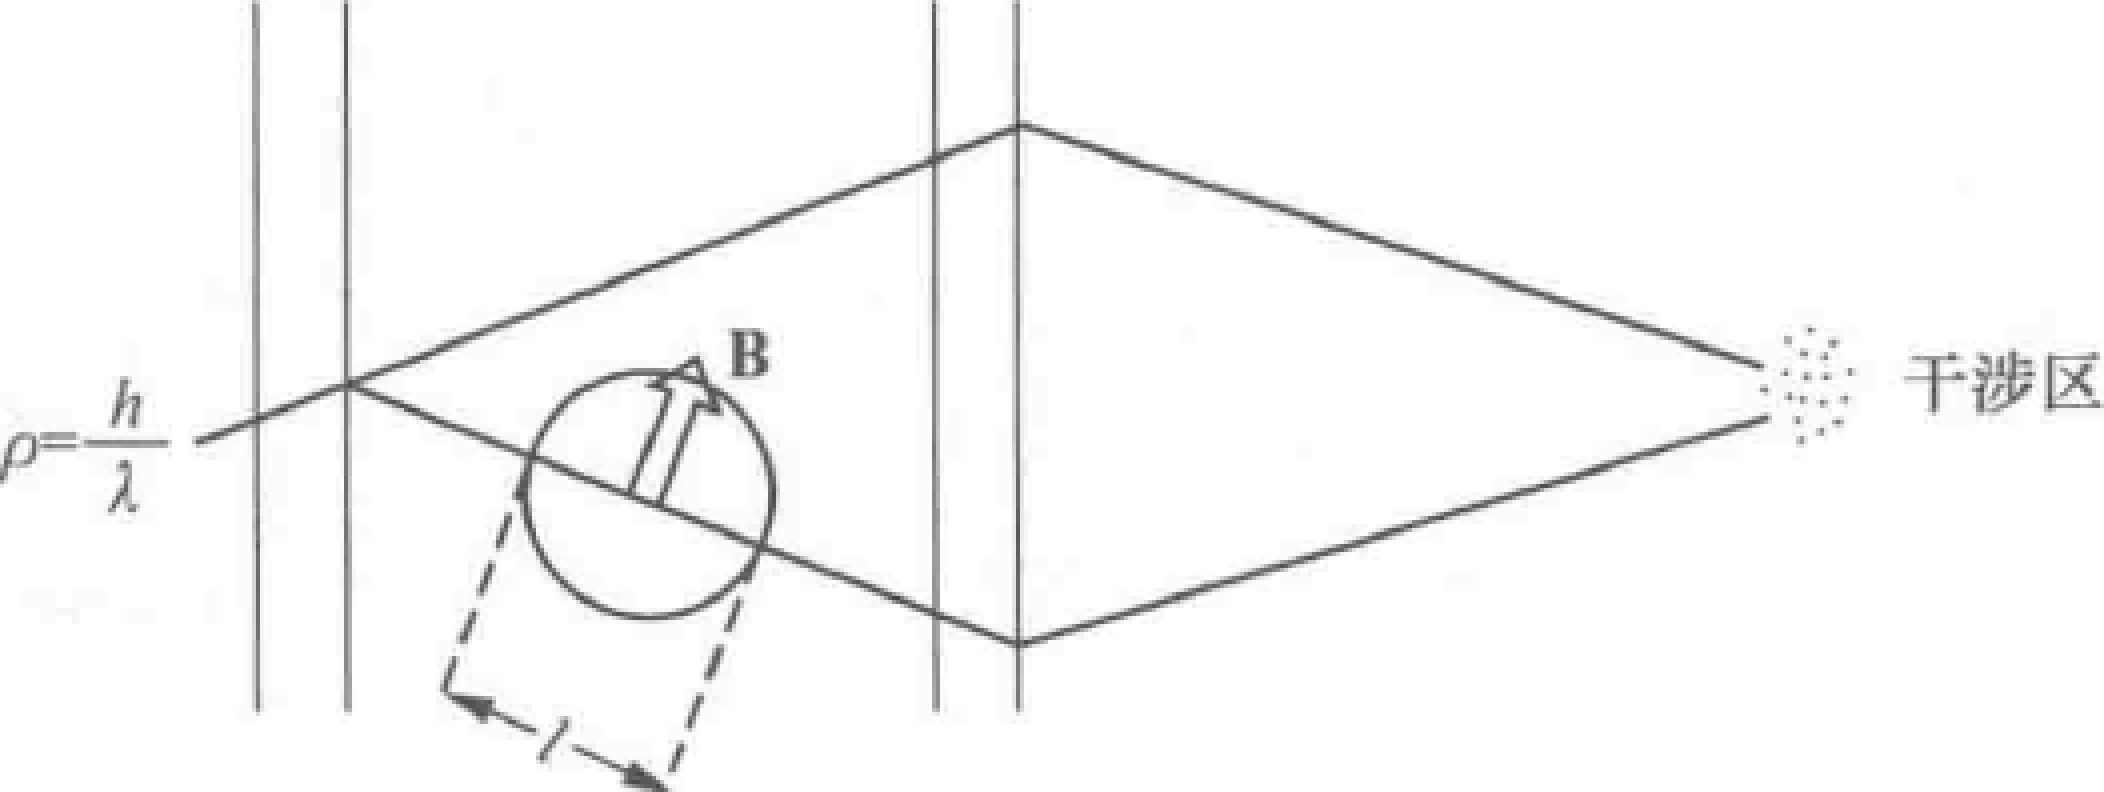
\includegraphics[width=.5\columnwidth]{4-9.png}
    \end{figure}
    证明在计数率中产生两个相继极大值的磁场差由下式给出
    \[
        \Delta B=\frac{4\pi\hbar c}{|e|g_n\bar{\lambda}l},
    \]
    其中 $g_s=(-1.91)$ 是中子磁矩. 单位为 $-e\hbar/2m_nc$. (假如你在 1967 年解出了这个问题的话, 你就会在 Physical Review Letters 上发表你的解!)
\end{prob}
\begin{pf}
    
\end{pf}
\end{document}